\section{Registro de mudanças no processo}


\begin{table*}[!h]
\centering
\caption{Mudanças no processo de Engenharia de Requisitos}
\label{Rotulo}
  \begin{tabular}{p{0.20\linewidth}p{0.25\linewidth}p{0.25\linewidth}}
  \hline
  Data  & Processos mudados & Versão Gerada\\
  \hline

  23/05/2015 & Macroprocesso e Subprocesso Executar Iteração & 2.0\\

  04/06/2015  & Macroprocesso & 3.0 \\

  \hline
  \end{tabular}
\end{table*}

Na versão 1.0 do processo, Figuras \ref{fig:Processo1} e \ref{fig:iteracao1}, atividades de gerência de mudanças e alguns \textit{gateways} foram acrescentados, também foi retirado o subprocesso
  Executar Release. Essas mudanças foram realizadas pois não havia um fluxo definido para quando
  surgissem novos Requisitos ao longo do processo e também não havia o relacionamento de volta entre os níveis do SAFe. O subprocesso foi retirado
  pois ele foi transformado em atividades no macroprocesso que seguiam a ordem correta de execução.

\textbf{Atividades acrescentadas:}

\textbf{Gerenciar mudanças no Programa}

  \textbf{Descrição}: Essa atividade consiste na gerência de mudanças no nível de programa, como o surgimento de novas 
  \textit{features}, novos épicos e novas histórias. Para cada um dos níveis de abstração requisitos essa atividade gera saída
  para uma atividade diferente.

  \textbf{Tarefas}:
  \begin{itemize}
   \item \indent \textit{Verificar o surgimento de novos requisitos}: Analisar se novos requisitos surgiram;

   \item \indent \textit{Analisar impacto da mudança}: Analisar o impacto e a relevância da mudança no projeto e decidir se será considerada
   ou descartada;

   \item \indent \textit{Registrar novos requisitos}: Registrar novos requisitos, se forem épicos realizar as atividades: Levantar Épicos e 
   Fazer reunião de validação dos épicos. Se forem \textit{features} realizar as atividades: Levantar Épicos e \textit{Features}  
   Fazer reunião de validação dos \textit{features} e se forem histórias realizar a atividade de Escrever histórias.
  
  \end{itemize}

  \textbf{Participantes}: Time\\

  \textbf{Entrada}: \textit{Backlog} do Programa e do Time \\

  \textbf{Saída}:  \textit{Backlog} do Programa e do Time \\
  

\textbf{Gerenciar mudanças na Iteração}

  \textbf{Descrição}: Essa atividade consiste na gerência de mudanças no nível de time, como o surgimento ou alocação de novas histórias.

  \textbf{Tarefas}:
  \begin{itemize}
   \item \indent \textit{Verificar o surgimento de novos histórias}: Analisar se novas histórias surgiram;

   \item \indent \textit{Verificar a necessidade de realocar histórias}: Analisar se será necessário realocar histórias em outra iteração;
   
   \item \indent \textit{Analisar impacto da mudança}: Analisar o impacto e a relevância da mudança na iteração e decidir se será considerada
   ou descartada;

   \item \indent \textit{Registrar novas histórias}: Registrar novas histórias e realizar a atividade de Escrever histórias.

   \item \indent \textit{Realocar histórias}: Realocar as histórias em outra iteração.
  \end{itemize}

  \textbf{Participantes}: Time\\

  \textbf{Entrada}: \textit{Backlog} do Time e da Iteração\\

  \textbf{Saída}:  \textit{Backlog} do Time e da Iteração\\
  
\begin{figure}[!htb]
\flushleft
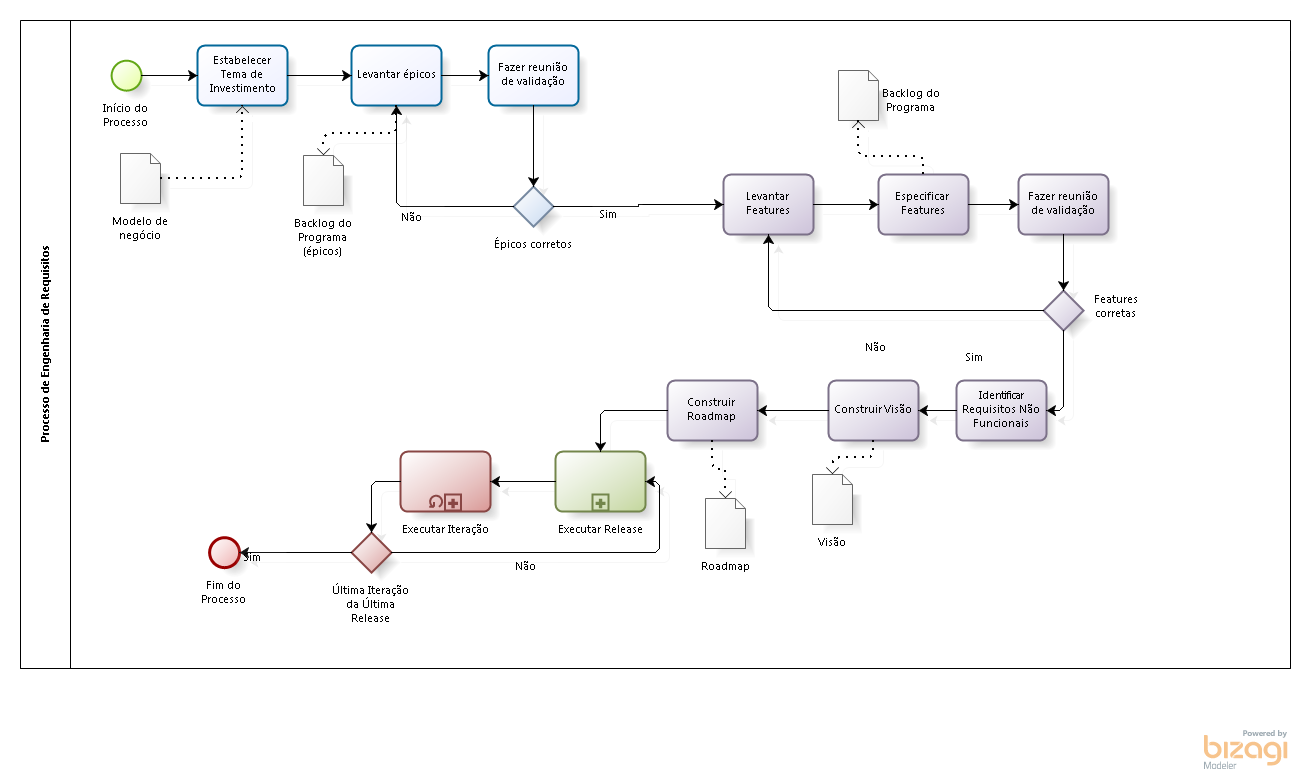
\includegraphics[scale=0.5]{figuras/processo1.png}
\caption{Processo de Engenharia de Requisitos - Versão 1.0}
\label{fig:Processo1}
\end{figure}

\begin{figure}[!htb]
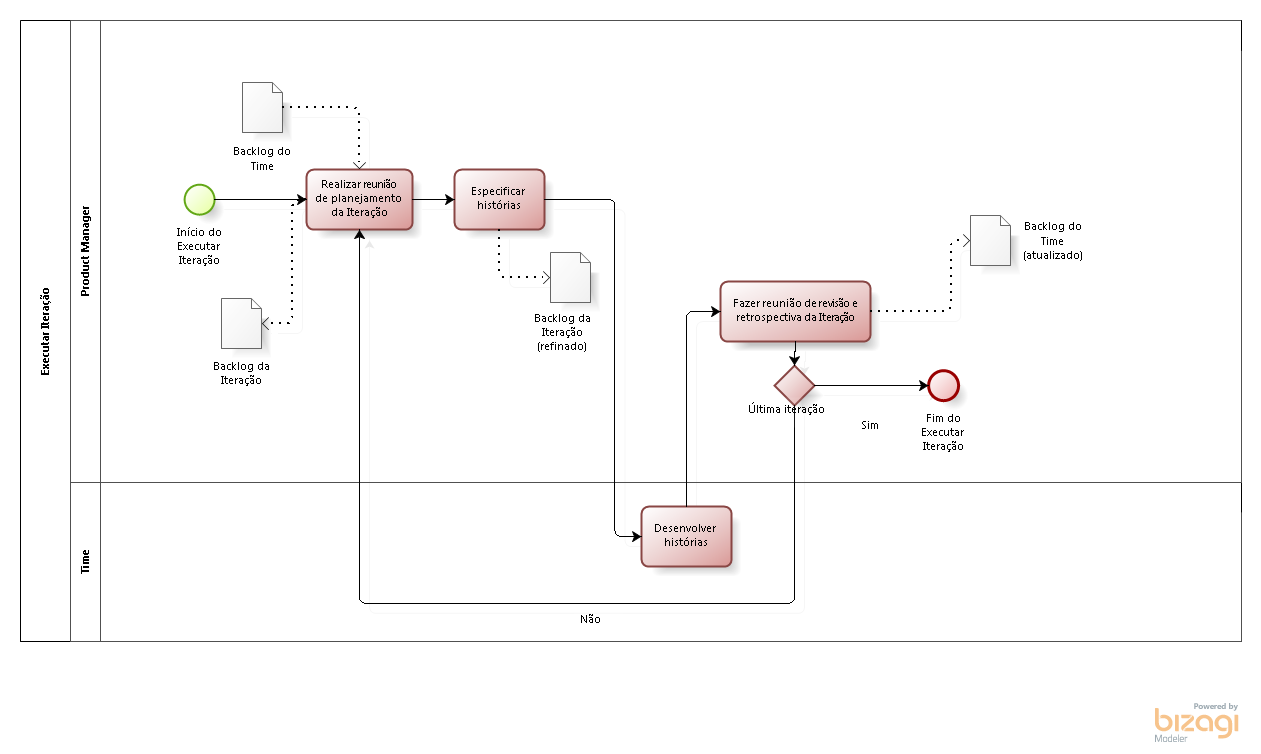
\includegraphics[scale=0.5]{figuras/iteracao1.png}
\caption{Suprocesso Executar Iteração - Versão 1.0}
\label{fig:iteracao1}
\end{figure}

\pagebreak
Na versão 2.0 do processo, Figura \ref{fig:Processo2}, atividades de validação dos épicos e \textit{features} foram mescladas às atividades de elicitação desses requisitos.
Essa mudança foi realizada, pois foi percebida que essas atividades poderiam ser tarefas, visto que em outros momentos do processo foi estabelecido assim.
Dessa forma, as atividades de Levantar Épicos e Levantar \textit{Features} ficaram da seguinte forma:

\textbf{Levantar Épicos}

  \textbf{Descrição}: Essa atividade consiste no levantamento dos épicos com o \textit{Product Manager} através do  \textit{Workshop} de Requisitos. \\

  \textbf{Tarefas}:

  \begin{itemize}
   \item \indent \textit{Fazer Workshop de Requisitos}: Reunião com o cliente e o time para levantar requisitos de mais alto nível. Consiste
   em uma técnica de elicitação definida no Capítulo \ref{tecnicas}.

   \item \indent \textit{Escrever Épicos}: A partir das anotações feitas no \textit{Workshop},
   escrever os épicos no \textit{Backlog} do Programa.
   
   \item \indent \textit{Validar Épicos}: Confirmar com o cliente se os épicos estabelecidos estão corretos.

   \item \indent \textit{Escrever Épicos}: Se houver alguma mudança solicitada pelo cliente, escrever os épicos
   refinados no \textit{Backlog} do Programa.
   
   \item \indent \textit{Manter Rastreabilidade}: Registrar na ferramenta cada épico como derivado do tema de investimento.

  \end{itemize}

  \textbf{Participantes}: \textit{Product Manager}, \textit{Scrum Master}, Time \\

  \textbf{Entrada}: Anotações do \textit{Workshop} \\

  \textbf{Saída}: Épicos Validados - \textit{Backlog} do Programa\\

\textbf{Levantar \textit{Features}}

\textbf{Descrição}: Essa atividade consiste em listar as \textit{Features}, a partir dos épicos ,
que são as tarefas ou os “serviços” que o sistema deve fornecer para atender as necessidades das partes interessadas.
Deve-se observar se as \textit{features} condizem com ou traduzem de forma clara os Épicos
definidos previamente, e se através delas é possível escrever as Histórias de Usuário.\\

\textbf{Tarefas}:

  \begin{itemize}
   \item \indent \textit{Listagem de \textit{Features}}:  Listar \textit{Features} a partir dos Épicos de Portfólio ou a partir de outras \textit{Features}.
   
   \item \indent \textit{Comparação \textit{Features}-Épicos}: Comparar as \textit{Features} e os Épicos, validando se as \textit{Features} expressam as iniciativas contidas nos Épicos;

   \item \indent \textit{Adição e Edição de \textit{Features}}: Adicionar novas \textit{Features} ou modificar as \textit{Features} já levantadas de acordo com as mudanças sugeridas no momento da Validação.

   \item \indent \textit{Validar \textit{Features}}: Confirmar com o cliente se as \textit{features} estabelecidas estão corretas. 
   
   \item \indent \textit{Manter Rastreabilidade}: Registrar na ferramenta de qual épico é cada \textit{Feature}.
   \end{itemize}

\textbf{Participantes}: \textit{Product Manager}, \textit{Scrum Master}, Time \\

\textbf{Entrada}: \textit{Backlog} do Programa (Épicos) \\

\textbf{Saída}:  \textit{Features} Validadas - \textit{Backlog} do Programa  \\


\begin{figure}[!htb]
\flushleft
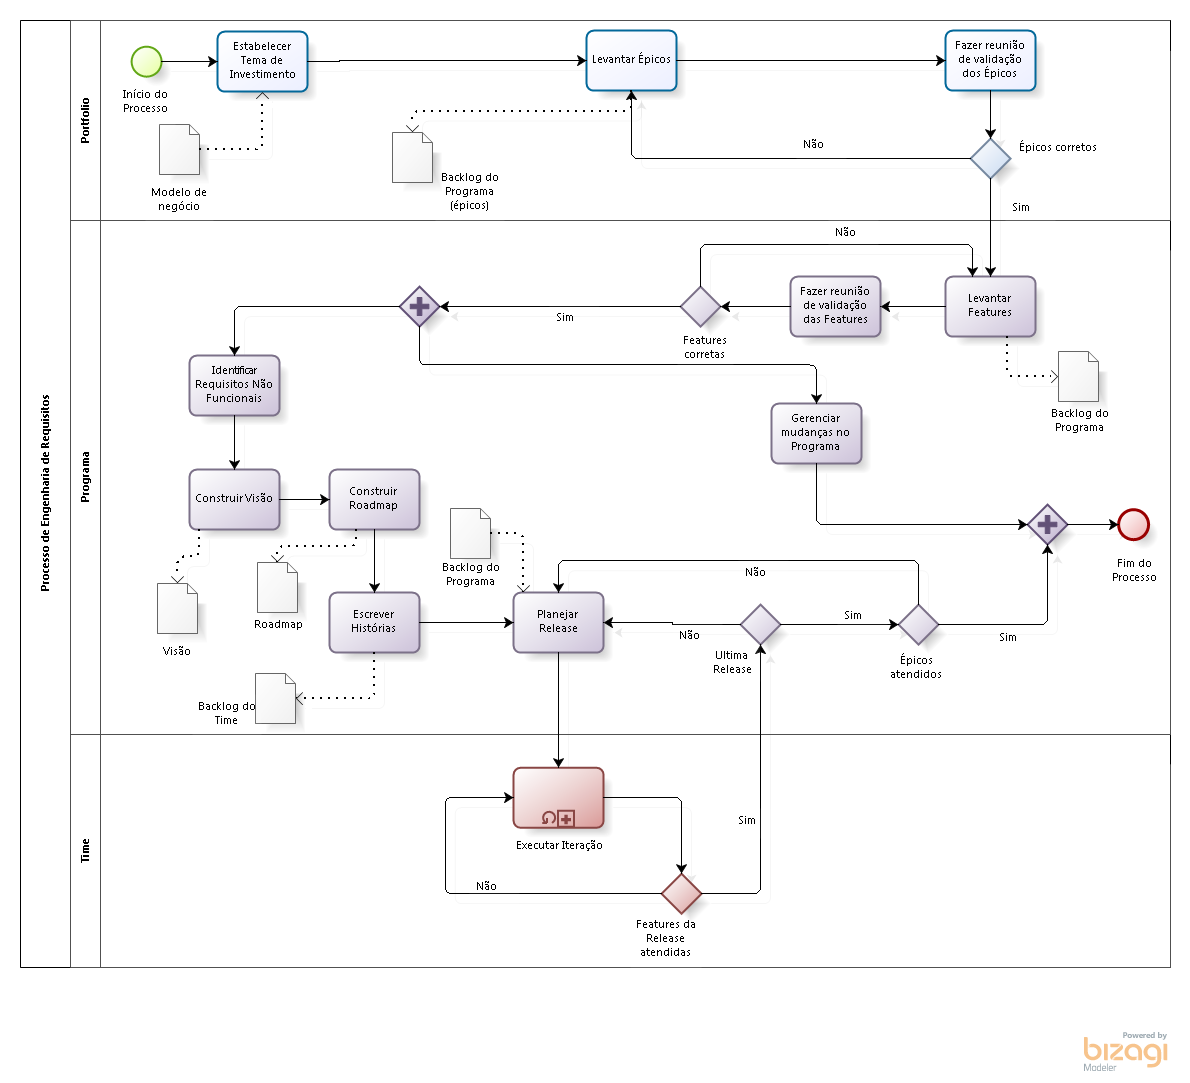
\includegraphics[scale=0.5]{figuras/processo2.png}
\caption{Processo de Engenharia de Requisitos - Versão 2.0}
\label{fig:Processo2}
\end{figure}
